\chapter{Ausblick}
\label{ch:ausblick}
Dieses Kapitel soll einen Überblick über größere Erweiterungen und Funktionen geben, durch die die Architektur, die
Webanwendung und die Smartphone-Apps erweitert und verbessert werden können.

Außerdem sollen Möglichkeiten aufgezeigt werden, welche die Arbeit mit Maschinen und künstlicher Intelligenz
vereinfacht. Dazu zählt unter anderem die Möglichkeit, eine direkte Verbindung zwischen Maschine und einem trainierten
Modell herzustellen.

Auch sind Themen, welche die klassische Container-Architektur verbessern für Erweiterungen interessant oder
auch Möglichkeiten zur schnelleren Vorhersage von Parametern und der Eingabe von Daten unter erschwerten Bedingungen.

\section{Kontinuierliches Lernen und Optimieren}
Zu Anfang soll eine Erweiterung aufgezeigt werden, welche die Möglichkeit bietet eine Maschine direkt mit einem
neuronalen Netz und einem trainierten Modell zu verbinden. Damit kann man die Maschine schneller und ohne menschlichen
Einfluss einstellen.

In der aktuellen Version der Architektur werden neuronale Netze auf der Basis von historischen Daten aufgebaut. Die so
trainierten Modelle werden in einem Deployment zur Verfügung gestellt und können ab dann Vorhersagen bearbeiten. Neue
Erkentnisse führen dazu, dass das Netz komplett neu trainiert werden muss.

Einfacher wäre es, wenn eine Maschine eine direkte Verbindung zu einem neuronalen Netz hätte und diesem kontinuierlich
neue Werte übergibt. Als Datensätze könnte zum Beispiel die Geschwindigkeit mit der die Maschine arbeitet übertragen
werden oder wie viele Produkte korrekt verarbeitet wurden -- also die bearbeiteten Produkte abzüglich dem Ausschuss.

Dies wäre umsetzbar, indem man die Maschine mit einem IoT-Gateway ausstattet, welches verschiedenste Messgrößen aus der
Maschine extrahiert und mittels MQTT an die IBM Cloud schickt. Bei dem IoT-Gateway könnte es sich um das
\textit{Rexroth IoT Device} handeln, welches diverse Treiber für die Maschinen der Robert Bosch GmbH mitliefert.

Diese Daten könnte man dann zusammenfassen und dem Machine Learning Service als Stream zur Verfügung stellen.

In einem Modeler Flow kann man diesen Stream dann aufgreifen und ein neues Modell auf Basis dieses Streams
kontinuierlich trainieren lassen. Dieses Modell könnte sich dann immer neuen Gegebenheiten automatisch anpassen. Die
Vorhersagen, die das trainierte Modell dann ausgibt, basieren dann auf den immer neuen Maschinenparametern und können
so die Produktivität erhöhen.

Eine Cloudant-Datenbank dient als Zwischenspeicher für die immer neuen Maschinenparameter, damit diese auch für
zukünftige Auswertungen bereitstehen.

Die \textit{Internet of Things Plattform} kümmert sich um die Verbindung zwischen Cloud und IoT-Gateway und um die
Übertragung der Daten von der Maschine in die Cloudant-Datenbank.

Die Abbildung~\ref{fig:ausblick_uebersicht} auf Seite~\pageref{fig:ausblick_uebersicht} zeigt eine Übersicht über eine
mögliche Architektur zur automatisierten Einstellung von Maschinenparametern.

\begin{figure}[h]
    \centering
    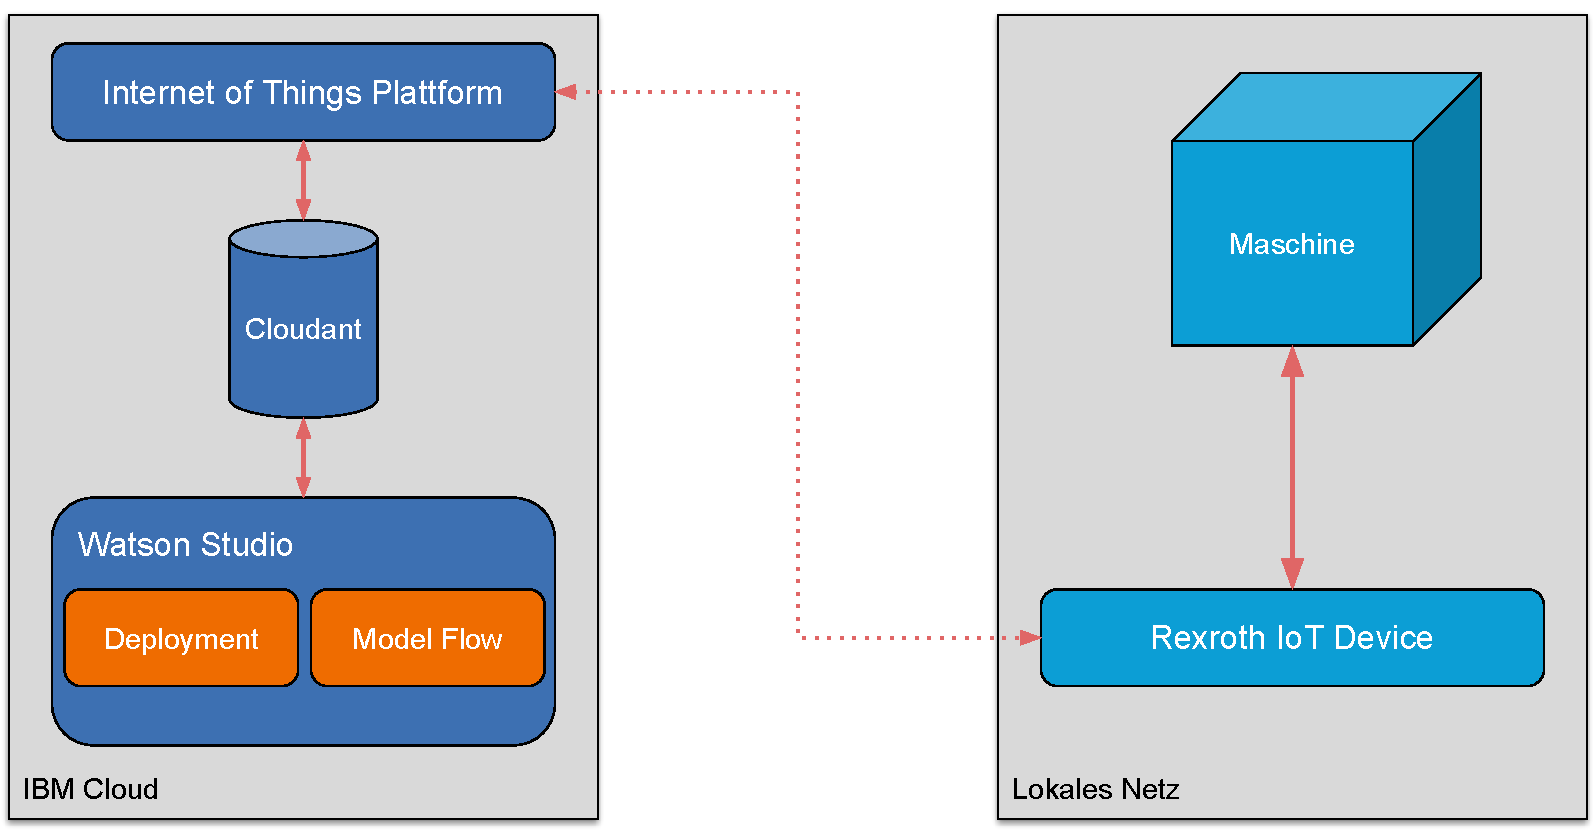
\includegraphics[width=\textwidth]{images/kapitel_6/architektur_uebersicht.pdf}
    \caption{Übersicht der Zielarchitektur}
    \label{fig:ausblick_uebersicht}
\end{figure}

Allerdings sind automatisierte Tests nicht immer und für jede Anwendung geeignet. Michael Lüttel von der Deutschen
Flugsicherung sagte auf der iqnite-Konferenz in Düsseldorf beispielsweise \enquote{Automatisierung macht nur dann Sinn,
wenn sie mehr Aufwände einspart als sie selbst
erzeugt.}\footnote{https://www.qz-online.de/news/uebersicht/nachrichten/vor-und-nachteile-von-automatisierten-software-tests-890130.html}.

\section{Function as a Service}
Zur Zeit ist in der Architektur ein Webservice mit dem trainierten Modell installiert und eingerichtet, welcher auf
einem Cloud Foundry Container basiert. Die Konfiguration und Instanthaltung des Containers übernimmt die IBM Cloud
automatisch und ohne menschliches Zutun.

Dieser Container wartet immerzu auf Anfragen an das eigene REST-Interface um eine Vorhersage zu erzeugen. Sollte über
einen Zeitraum keine Anfrage ankommen, verbraucht dieser Container allerdings kostspielige Ressourcen wie zum Beispiel
Arbeitsspeicher, da er immer betriebsbereit sein muss.

Um diesem Problem entgegenzuwirken existieren Services für den Serverlosen Betrieb (englisch Serverless Computing).
Diese heißen \textit{Functions as a Service} (kurz FaaS) und sind in der IBM Cloud unter dem Namen \textit{Functions}
zu finden. Die Funktionsweise dieses Services basiert auf Apache OpenWhisk.

Dieser Service stellt online eine Ordnerstruktur für den Kunden bereit, in der er selbstgeschriebenen Quellcode
hinterlegen kann. Dabei werden alle gängigen Programmiersprachen und Laufzeiten unterstützt.

Nachdem man den Quellcode hochgeladen hat, kann man sogenannte \textit{Trigger} definieren. Ein Trigger steht für ein
Ereignis, welches an einem Provider stattfindet. Dies kann zum Beispiel ein Aufruf eines Endpunktes sein, ein neuer
Eintrag in einer Datenbank, eine Push-Benachrichtigung oder andere Funktionen, welche man selbst definieren kann.

In Abbildung~\ref{fig:ausblick_functions} auf Seite~\pageref{fig:ausblick_functions} ist der Wizzard der Functions zu
sehen. Hier kann man die Trigger definieren und die Aktionen einstellen, welche ausgeführt werden sollen.

\begin{figure}[h]
    \centering
    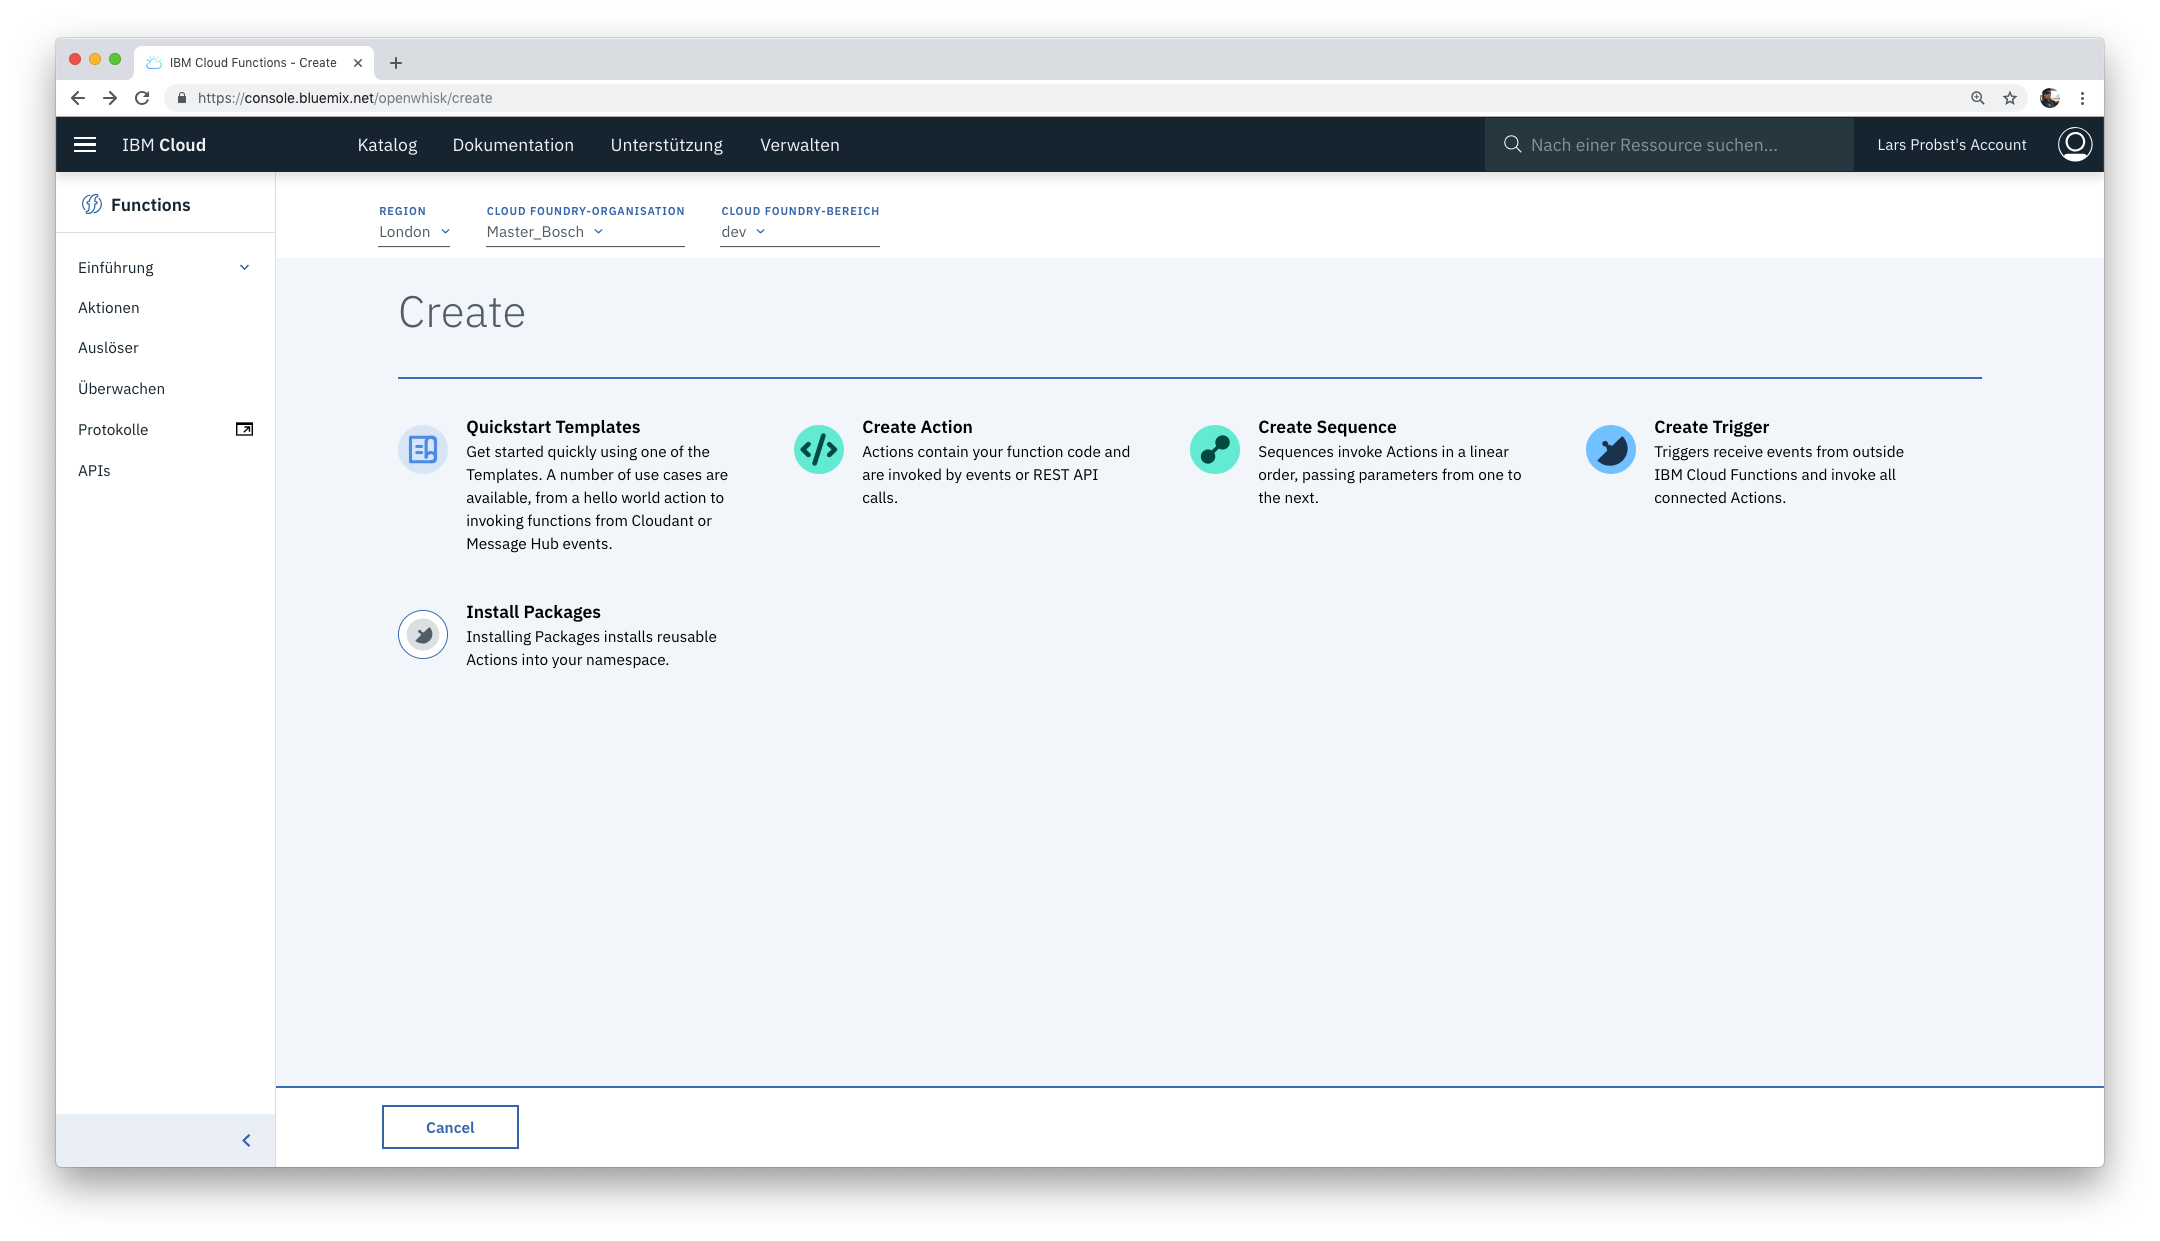
\includegraphics[width=\textwidth]{images/kapitel_6/functions_wizzard.png}
    \caption{Einstellungen für die Functions}
    \label{fig:ausblick_functions}
\end{figure}

Sofern dieses Ereignis eintritt, startet der Service \textit{Functions} eigenständig den selbstgeschriebenen Quellcode
und führt ihn aus. Dabei wird ein Cloud Foundry Container gestartet, eine Runtime für den Quellcode eingerichtet und
dieser dann ausgeführt.

Wenn der Quellcode fertig abgearbeitet ist, fährt der Container selbstständig herunter und die benötigten Ressourcen
werden nicht weiter beansprucht.

Mit der Hilfe dieser Funktion kann man das online in der Cloud trainierte Modell mit dem TensorFlow-Wrapper in den IBM
Service Functions laden und diesen immer dann ausführen lassen, wenn ein Request ankommt.

So kann man Geld für die ansonsten ständig belegten Ressourcen des Containers sparen und muss sich um keine Container
mehr kümmern.

\section{Offline Modus}
Anstatt das trainierte Modell aus der Cloud in einem TensorFlow-Wrapper einzurichten um es anschließend mit einer
REST-Schnittstelle zu versehen kann man es auch direkt und nativ im Browser (bisher nur Chrome von Google) einbetten.

Dafür muss man das Frontend dahingehend erweitern, dass Anfragen davon nicht an eine online REST-Schnittstelle geschickt
werden, sondern direkt an das im selben Verzeichnis gespeicherte trainierte Modell.

Das Trainieren des Modells kann trotzdem in der Cloud geschehen. Man muss es anschließend aber herunterladen und in der
Angular-Anwendung verfügbar machen. Mittels TensorFlow-Bibliotheken kann man eine Anfrage dann direkt an das lokale
Modell stellen und erhält die Vorhersagen schneller.

Auch wird in dieser Version keine Internetverbindung für Vorhersagen benötigt. Nachdem die Webseite einmal
heruntergeladen ist, können Anfragen sogar im offline Modus geschehen und die Anwendung steht komplett offline zur
Verfügung.

\section{Machine Learning für Smartphones}
Auch kann das trainierte Modell nicht nur im Browser zur Verfügung gestellt werden, sondern auch in einer nativen
Android"~ oder iOS-App.

Dafür existieren im Android-SDK oder in Xcode Funktionen für den direkten Zugriff auf trainierte neuronale Netze. Dabei
muss das Modell nicht schon im Voraus trainiert sein. Es kann auch direkt auf dem Smartphone in Echtzeit passieren.

Unter Android steht beispielsweise die \textit{Neural Networks API} bereit. In dieser kann man die Testdaten mit der APK
ausliefern und selbst trainieren lassen. Dies hat den Vorteil, dass man keine eigenen Ressourcen für das Training und
für das Bereistellen eines Backends aufbringen muss.

Auch wäre es möglich die Android-App beim Start die aktuellsten Trainingsdaten herunterladen zu lassen um dann das
neuronale Netz auf Basis der neuen Daten trainieren zu lassen.

Nachdem das neuronale Netz auf dem Smartphone trainiert ist, kann man Anfragen direkt aus der selbst geschriebenen App
stellen und benötigt keine Internetverbindung mehr.

Diese Variante funktioniert allerdings nur bei nativen Apps. Da es sich allerdings bei der WebView-App um eine native
App handelt, welche die Webseite herunterlädt, kann man diese um die Funktion der lokalen neuronalen Netze erweitern.

Da es aus einer WebView-App möglich ist, den HTML"~ sowie den JavaScript-Code zu manipulieren ist es lediglich notwendig
die Funktion hinter dem \textit{Senden}-Button so abzuändern, dass man die eingegebenen Daten nicht an das Backend
schickt, sondern an das lokal trainierte Modell.

So kann das normale Frontend weiterhin mit dem Backend kommunizieren und die Smartphone-Apps nutzen eigene trainierte
Modelle zur verbesserten Performance. Trotzdem kann das Frontend erweitert werden und die Smartphone-Apps müssen nicht
neu gebaut werden.

\section{AI OpenScale}
\label{ai_openscale}
Der Service AI OpenScale aus der IBM Cloud kann den internen Aufbau eines trainierten neuronalen Netz anzeigen und
nachvollziehbar darstellen. Dabei ist es unter anderem Möglich zu verstehen, wie das neuronale Netz auf die Vorhersage
kommt und zu welcher Wahrscheinlichkeit es sich sicher ist.

Dabei muss man eine Datenbank mit dem Watson Studio Service verbinden, damit diese alle Tätigkeiten des neuronalen
Netzes und des trainierten Modells aufzeichnet. Diese Aufzeichnung passiert nach der Einrichtung automatisch.

Nachdem man mehrere Vorhersagen durchgeführt hat, zeigt der AI OpenScale Service zahlreiche Informationen an und
visualisiert dem Nutzer, wie die Vorhersagen zustandegekommen sind.

Auf der Produktseite\footnote{https://www.ibm.com/cloud/ai-openscale} des Services sind zahlreiche Beispiele und Videos
zu sehen, welche die Funktionsweise veranschaulichen.

Der Service wurde unter dem Gesichtspunkt \texttt{Transparenz} entwickelt. Er soll die Angst vor neuronalen Netzen
eindämmen in dem nachvollziehbar wird, warum und vorallem wie Ergebnisse zustandekommen.

\section{Audit mit Blockchain}
Aktuell muss der Maschineneinsteller für jede Auslieferung einer KWE der Robert Bosch GmbH ein Excel-Dokument ausfüllen
in dem diverse Tests, eingestellte Parameter und Funktionen der Wiegeeinheit festgehalten und überprüft werden.

Dieses Dokument dient zur Validierung der korrekten Funktionsweise der Waage und man kann damit zu jedem späteren
Zeitpunkt, nach erfolgter Auslieferung, die korrekte Funktion zur damaligen Zeit beweisen.

Das Dokument dient ebenfalls zur Absicherung der Robert Bosch GmbH gegenüber dem Gesetzgeber, dass die Wiegeeinheit
korrekt geeicht wurde und muss über den kompletten Lebenszyklus der Maschine aufbewart werden.

Aus diesem Grund ist es wichtig, dass das Dokument nach der Anfertigung weder verschwindet, noch nachträglich verändert
oder manipuliert wird.

Zum Speichern und zum Schutz vor unberechtigter Veränderung von Informationen existiert seit dem Jahr 2008 eine neue
und sichere Speichermöglichkeit -- die Blockchain.

Sowohl das WallStreet
Journal\footnote{https://www.wallstreet-online.de/nachricht/10475136-ey-announces-blockchain-audit-technology} als auch
die Seite des Blockchain-Wikipedia-Eintrags\footnote{https://de.wikipedia.org/wiki/Blockchain} zeigen zahlreiche
Vorschläge für den automatisierten Audit-Vorgang im Unternehmensbereich.

Dabei ist die Idee, die eingestellten Parameter der Maschine, bevor sie zum Kunden ausgeliefert wird, in einer
Blockchain zu speichern. Die Architektur der Blockchain stellt anschließend sicher, dass nach erfolgreichem anlegen
eines Blockes, welcher mit den Informationen gefüllt ist, dieser vor fremden Zugriffen und manipulationen geschützt ist.

Allerdings muss man dabei beachten, dass das Auslesen der Informationen aus der Maschine und das Übertragen der Daten
an den Blockchain-Knoten so abgesichert sein muss, dass keine fremde Person diese Daten verändern kann.

In einem darauf aufbauenden Schritt könnte ein neuronales Netz wiederkehrend mit den Maschinenparametern versorgt
werden, um sich selbst neu einzustellen. Die daraufhin veränderten Parameter und darauf aufbauenden Tests müssten
automatisiert an den Block der Ureinstellung gehängt werden.

Damit wäre es später möglich, dass man Änderung nachvollziehen und die daraus resultierenden Verbesserungen zu jedem
Zeitpunkt einsehen kann.

Auch wäre es so möglich, gegenüber dem Gesetzgeber nachvollziehbar beweisen zu können, wann und zu welchen Parametern
die Maschine anders konfiguriert wurde und mit welchen Parametern sie anfangs an den Kunden ausgeliefert wurde.

Die Blockchain übernimmt damit die Funktion der alten Excel-Tabelle und es ist zu jedem Zeitpunkt sichergestellt, dass
die Informationen jeder einzelnen Waage sicher an einem Ort aufbewart und Änderungen protokolliert sind.